\section{Feil og feilanalyse: FMECA}
\label{sec:fmeca}


\subsection{FMECA intro}

FMECA står for FeilMode Effekt (C)Konsekvens/kritikalitet Analyse og er en metodikk for å analysere feilmoder. Det er en systematisk og strukturert metode med fast oppsett, hvor resultatet presenteres i en FMECA-tabell, se eksempel i figur \ref{fig:fmeca_propell}.

\begin{figure}[H]
    \centering
        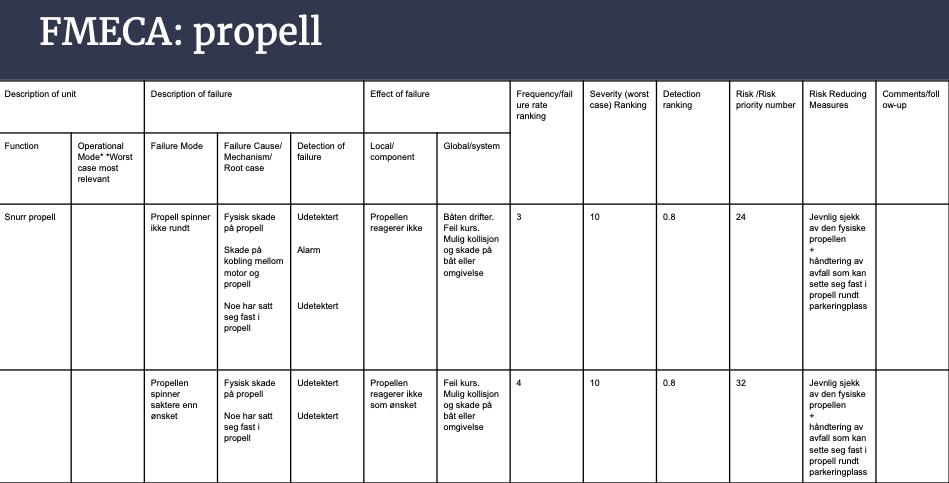
\includegraphics[width=\textwidth]{figures/FMECA/Skjermbilde 2021-11-24 kl. 09.54.55.png}\\
        \caption{Eksempel på FMECA-tabell for propell på båt.}
        \label{fig:fmeca_propell}
\end{figure}

FMECA brukes til å identifisere alle potensielle feilmoder av forskjellige deler av et system, konsekvensene av disse feilmodene, og hvordan vi kan unngå eller minske effekten av feilene.

FMECA er en teknikk for å identifisere, prioritere og eliminere potensielle feil fra et system, design eller prosess før de når kunden.

\subsection{Bakgrunn}
\begin{itemize}
    \item FMECA er en av de tidligste formene for feilanalyse, og ble utviklet av det amerikanske militære.
    \item FMECA blir mest brukt i reliabilitetsanalyse i tidlig stadie i produkt/system-utvikling, vanligvis under konsept- og tidlig design-fase for å sikre at alle potensielle feilmoder har blitt evaluert og at man har på plass riktige tiltak for å eliminere disse feilene.
\end{itemize}

\subsection{Metode}

\textbf{I forkant av FMECA-gjennomføring}

\begin{itemize}
    \item[\textbf{1:}] Definer systemet som skal analyseres.
    \begin{itemize}
        \item Systemgrenser (hva skal inkluderes og ikke)
        \item 
    \end{itemize}
\end{itemize}



\begin{figure}[H]
    \centering
        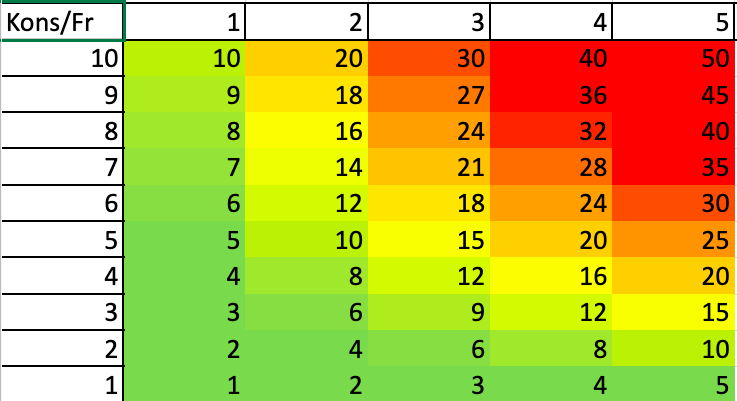
\includegraphics[width=\textwidth]{figures/FMECA/Skjermbilde 2021-11-24 kl. 09.47.58.png}\\
        \caption{Eksempel på risikomatrise brukt i FMECA.}
\end{figure}